\section{Learned lens ladders: an audit}
\label{sec:learned}

The most natural way to choose a lens without looking at coordinates is to learn it from the kernel.
This section applies the pipeline with lenses learned by spectral clustering to four substrates and audits the result.
The finite metrics are valid and respond to constraints in the expected way, but the ladders do not meet the coherence criterion at their fine levels, and for two of them we prove that no choice of prototypes can change this.

\subsection{Substrates and learned ladders}
\label{sec:substrates}

\begin{itemize}[leftmargin=*]
\item \textbf{Grid.} The lazy walk on the open $25\times25$ grid ($625$ states): stay with probability $\tfrac12$, otherwise move to a uniformly chosen valid cardinal neighbour. Boundary states therefore have degree three or two.
\item \textbf{Sphere $k$NN.} $500$ points sampled on the unit sphere are used only to build a weighted $10$-nearest-neighbour graph with Gaussian weights ($\sigma=0.5$, self-loop $10^{-6}$), which is symmetrized and row-normalized. The coordinates are not used anywhere else.
\item \textbf{Gasket.} The lazy walk on the level-$5$ Sierpi\'nski gasket graph ($366$ states), stay probability $\tfrac12$.
\item \textbf{Gated grid.} The grid walk with every westward move removed and each row renormalized (``east'' gating at full strength).
\end{itemize}
Lens ladders with $m\in\{4,8,16,32,64,128\}$ macro states are learned from each kernel.
The spectral coordinates~\cite{CoifmanLafon2006,vonLuxburg2007} are the six nontrivial lowest eigenvectors of the normalized Laplacian $I-D^{-1/2}SD^{-1/2}$ of the symmetrized kernel $S=\tfrac12(P+P^{\mathsf T})$ (with $D$ its degree matrix), each row normalized to unit length; they are clustered into $128$ groups by a seeded $k$-means routine~\cite{Lloyd1982}, and coarser levels are obtained by merging cluster centroids, which makes the ladder nested by construction.
All runs use $\tau=5$, uniform prototypes, weight averaging, floor $\eta=10^{-12}$ and threshold $\varepsilon_{\mathrm{edge}}=10^{-15}$.
Because the coordinates are computed from $P$ itself, the lens extracts slow modes of the symmetrized dynamics rather than an ambient coordinate system; for the non-reversible gated grid these need not be eigenmodes of $P$.
It is still an observer's choice, and different choices can produce different geometries.

\subsection{What the audits show}

\begin{figure}[t]
\centering
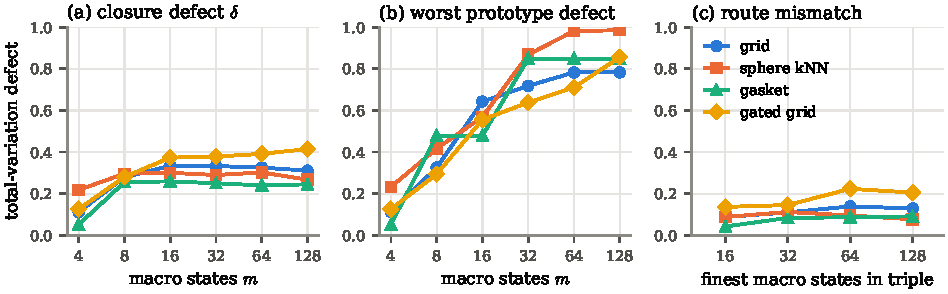
\includegraphics[width=\linewidth]{figures/fig_learned_audit.pdf}
\caption{Audits of the learned ladders at each level. (a) For $m\ge8$ the closure defect $\delta$ remains substantial, between $0.24$ and $0.42$. (b) The worst prototype defect never decreases with resolution (it plateaus at some levels) and reaches $0.78$--$0.99$ at the finest level. (c) Route mismatch on fine prototype inputs, for each nested triple, indexed by its finest level. All values are total-variation distances in $[0,1]$.}
\label{fig:learned-audit}
\end{figure}

\begin{table}[t]
\centering
\small
\caption{Learned ladders at the finest level ($m=128$, $\tau=5$). $\delta$: closure defect; $\bar s$, $\max s$: mean and worst prototype defect; $\RM$: largest route mismatch over nested triples; Dist: largest fitted raw distortion over adjacent levels (cost units); $\bar d$: mean finite off-diagonal distance; $n_\infty$: number of infinite distances. Floating computation.}
\label{tab:learned}
\begin{tabular}{@{}lrrrrrrrr@{}}
\toprule
Substrate & states & $\delta$ & $\bar s$ & $\max s$ & $\RM$ & Dist & $\bar d$ & $n_\infty$ \\
\midrule
Grid & 625 & 0.311 & 0.625 & 0.783 & 0.139 & 6.05 & 13.29 & 0 \\
Sphere $k$NN & 500 & 0.267 & 0.855 & 0.985 & 0.112 & 5.27 & 9.00 & 0 \\
Gasket & 366 & 0.245 & 0.641 & 0.849 & 0.091 & 8.35 & 19.37 & 0 \\
Gated grid & 625 & 0.415 & 0.615 & 0.856 & 0.223 & 11.25 & 13.42 & 0 \\
\bottomrule
\end{tabular}
\end{table}

\Cref{fig:learned-audit,tab:learned} report the audits.
Every macro graph is connected and every distance finite, so each level carries a genuine finite metric.
The closure defect, however, stays between roughly a quarter and two fifths at all but the coarsest levels, and the worst prototype defect never decreases as the resolution increases.
At the finest level a walker started from the worst block's prototype leaves the block with probability $0.78$ on the grid, $0.85$ on the gasket and $0.99$ on the sphere.
These blocks contain only three to five microstates on average, which is small compared with the spread of a five-step walk.
In the terms of \cref{def:coherence}, these ladders do not provide coherent layers at their fine levels; their finite metrics are measurements, not evidence of a stable emergent geometry.

\subsection{Reweighting prototypes cannot repair persistence}

One might hope to lower the defects by choosing better prototypes for the same partition.
For persistence, the best possible choice can be computed exactly.

\begin{theorem}[Optimal prototypes for a fixed partition]
\label{thm:prototype-obstruction}
Fix $P$, $\tau$ and a partition with coarse matrix $C$, and let $B=P^{\tau}C$.
Over all stochastic prototype matrices $U$ supported on the fibres,
\begin{equation}
\min_U\ \max_{x}\ s_U(x)\;=\;\max_x\Bigl(1-\max_{z\in f^{-1}(x)}B_{zx}\Bigr),
\end{equation}
and the minimum is attained by point-mass prototypes.
\end{theorem}

\begin{proof}
By \cref{prop:closure-basic}(iii), $s_U(x)=1-(UB)_{xx}=1-\sum_{z\in f^{-1}(x)}u_x(z)B_{zx}$.
The sum is a convex average of the return probabilities $B_{zx}$ over the fibre, so it is at most their maximum, which a point mass at a maximizing microstate attains.
The fibres are disjoint, so these choices can be made independently.
\end{proof}

\provenance{Lean: \lean{macro_return_le_fiber_bound} and \lean{prototype_defect_ge_fiber_escape} in \lean{PrototypeObstruction.lean} give the lower bound; attainment is the elementary construction above. Exact computation: the canonical values below are rebuilt from the recorded partitions by integer recurrence.}

For the canonical finest partitions the right-hand side is computed exactly from integer five-step recurrences (common denominators $24^5$ for the open grid and $8^5$ for the gasket).
On the grid it equals $6411/8192\approx0.7826$, attained on a two-state fibre whose states both return with probability $1781/8192$; on the gasket it equals $6957/8192\approx0.8492$, attained on a singleton fibre.
Uniform prototypes already achieve these minima, so no reweighting can lower the worst grid or gasket defect.
The result is conditional on the recorded partitions (it does not certify the eigensolver that produced them) and concerns persistence only; it is not a lower bound on $\delta$.
For the sphere the reported $0.985$ refers to uniform prototypes.
With the kernel, the stage $\tau=5$ and the persistence criterion held fixed, persistence can only be restored by changing the lens, and \cref{sec:constructed} does so.

\subsection{Constraints deform the metric at a fixed lens}
\label{sec:anisotropy}

Constraints change which moves are feasible, and so they should change the geometry.
Comparing the canonical grid and gated-grid runs confounds two effects, because the learned partition changes too.
To isolate the dynamical effect we hold the finest canonical grid lens and its prototypes fixed and replace only the micro kernel by its gated version.
The largest change in a macro transition probability is then $0.231$ and the largest change in a macro distance is $2.42$.
For pairs of microstates four lattice steps apart, the ratio of mean horizontal to mean vertical macro distance moves from $0.984$ without gating to $1.087$ with it.
The induced metric is thus deformed by the constraint at a fixed interface.
The horizontal and vertical directions here are readouts supplied by the known substrate, used only to describe the deformation.

\subsection{Local obstructions to Euclidean embedding}
\label{sec:nonembedding}

Is a learned metric locally Euclidean?
A reconstruction algorithm that fits poorly does not answer this, because a different algorithm might fit better.
A certificate must rule out every fit.
For four points in any real inner-product space,
\begin{equation}
d_{01}^2+d_{23}^2\;\le\;d_{02}^2+d_{03}^2+d_{12}^2+d_{13}^2,
\label{eq:quadrilateral}
\end{equation}
because the difference of the two sides is $\|p_0+p_1-p_2-p_3\|^2$.
If certified lower bounds on the ``diagonals'' $d_{01},d_{23}$ and upper bounds on the four ``sides'' violate~\eqref{eq:quadrilateral} even after every distance is perturbed by $\epsilon$, then no embedding of the four points into any inner-product space, of any dimension, reproduces all six distances to within $\epsilon$.

\provenance{Lean: \lean{hilbert_quadrilateral} and \lean{no_hilbert_uniform_approximation} in \lean{EuclideanObstruction.lean}. Exact computation: macro probabilities are rebuilt in integer arithmetic from the recorded partitions, shortest paths are found by exact multiplicative search, and logarithms are enclosed in rational intervals.}

Applied to a neighbourhood of a centre and its $24$ nearest macro neighbours, this yields exact witnesses for the canonical learned metrics: no inner-product fit of the selected gasket patch is accurate to within $9.1\%$ of the patch radius, and none of the grid patch to within $5.6\%$.
Similar witnesses hold for a family of substrate sizes in which a single learned partition with $m=\min(256,\max(16,\lfloor n/3\rfloor))$ macro states is used (grids of $49,121,361,1089$ states with $m=16,40,120,256$, and gaskets of $42,123,366,1095$ states with $m=16,41,122,256$; patches have $\min(24,m-1)$ neighbours): the excluded relative errors are $6.2$--$8.6\%$ for grids and $9.4$--$11.3\%$ for gaskets. For the smallest sizes the patch covers most of the macro graph, so these are global rather than local statements.
The essential point is that the grid fails as well.
Failure of local Hilbert embeddability in a finite learned metric does not by itself indicate a fractal; it is equally a feature of the $L^1$-like metrics that grid walks produce (\cref{sec:grid}).

\subsection{Dimension proxies}

Two finite proxies for dimension are standard: the slope of the logarithm of mean ball size against the logarithm of the radius in the induced metric (ball growth), and the slope of the packaged entropy against the logarithm of the inverse typical spacing across the ladder (information dimension)~\cite{Renyi1959DimensionEntropy,CoverThomas2006,Falconer2003Fractal}.
On a $20\times20$ grid and the level-5 gasket with the canonical ladder, the ball-growth slopes are $1.67$ and $1.39$ and the information slopes $4.66$ and $2.07$.
Replacing the distance $d$ by $\sqrt d$ roughly doubles the ball-growth slopes ($3.34$ and $2.78$), so these numbers depend on the cost convention and cannot be identified with the dimensions $2$ and $\log3/\log2\approx1.585$.
In the size family above (single partition, $m=\min(256,\max(16,\lfloor n/3\rfloor))$), the grid ball-growth slope stays between $1.61$ and $1.77$ and the gasket slope between $1.28$ and $1.38$; the contrast persists, but it is not a dimension estimate.
An exact dimension requires a limit object, which \cref{sec:gasket} constructs.
